\section{Evaluation}
\label{sec:eval}

\TODO{Pierre: Add explicit evaluation questions at the beginning. Right now the evaluation reports results without clearly connecting each subsection to the main claims made by ToFU. The questions should cover the applicability of the sanitizer corpus, semantic bug discovery, runtime filtering, fuzzing effectiveness, and real-world vulnerability discovery. You can phrase these based on the experiments that are already available.}

We structure our evaluation around the following research questions:

\noindent\textbf{RQ1 --- Sanitizer applicability.} To what extent can \project{}'s sanitizer corpus be mapped to the semantics exposed by real-world LLM tools?

\noindent\textbf{RQ2 --- Semantic bug detection.} Can \project{} detect violations of tool-specific semantic contracts that would not necessarily manifest as conventional crashes or schema violations?

\noindent\textbf{RQ3 --- Runtime filtering.} Can \project{} distinguish security-relevant semantic violations from benign runtime behavior observed during normal tool execution?

\noindent\textbf{RQ4 --- Fuzzing effectiveness.} Does coverage-guided mutation over schema-valid invocations reach the tool code paths that the selected sanitizers are meant to exercise, and does it surface semantic violations in real-world, publicly deployed tools?

We address RQ1 in Section~\ref{sec:eval-tools}, RQ2 and RQ3 in
Section~\ref{sec:eval-vulns}, and RQ4 in Section~\ref{sec:eval-coverage}.

\TODO{Pierre: Add an experimental setup subsection using the information already available. Report the machine configuration, operating system, Python and Node.js versions, number of cores used for each run, timeout policy, and fuzzing budget. Also state whether each reported result comes from a single run or multiple runs so that the methodology is explicit.}

% TODO(Nazmul): In a later evaluation revision, add repeated fuzzing trials for
% stochastic experiments and report an aggregate result and variance.

% TODO(Nazmul): In a later evaluation revision, add baseline and ablation
% experiments. At minimum compare full ToFU against ordinary Atheris or
% equivalent schema-guided fuzzing without semantic sanitizers and semantic
% runtime oracles. Separately evaluate the contribution of LLM seeding, the
% Seed Bank, sanitizer specialization, and semantic runtime checking.

\subsection{Tool selection}
\label{sec:eval-tools}
We evaluated our approach on 569 tools collected from 11 open-source
repositories. The repositories were chosen by taking the top MCP servers listed on https://github.com/mcp that could be fuzzed locally with simple setup. In addition, we've taken the first result when searching for "AI tool" on GitHub. 

\TODO{Pierre: The repository selection methodology needs to be reproducible. Define exactly what top MCP servers means, give the date on which this ranking was collected, report the initial candidate set if that information is available, and state the inclusion and exclusion criteria. In particular, define what could be fuzzed locally with simple setup means.}

\TODO{Pierre: The first result when searching for AI tool on GitHub is difficult to defend as a systematic sampling criterion. If this repository was included for a specific reason, explain that reason and treat it as an intentionally selected target rather than presenting the GitHub search result as part of a systematic sampling methodology.}

Table~\ref{tab:evaluation_repositories} details the complete breakdown of the 11 target repositories, spanning both native Python tools and Node.js MCP servers.

\begin{table}[h]
\centering
\caption{Breakdown of the 11 evaluated target repositories and tools.}
\label{tab:evaluation_repositories}
\begin{tabular}{lllr}
\hline
\textbf{Repository} & \textbf{Runtime} & \textbf{Description / Category} & \textbf{Tools} \\
\hline
\texttt{tools-main}          & Python     & Standalone Agent Tool Suite    & 412 \\
\texttt{pmb}                 & Python     & Memory \& Cognitive Graph MCP  &  68 \\
\texttt{serena}              & Python     & Workspace \& Coding Agent MCP  &  43 \\
\texttt{memo}                & Python     & Knowledge Graph \& Memory MCP  &  17 \\
\texttt{basic-memory}        & Python     & FastMCP Semantic Note Storage  &   9 \\
\texttt{markitdown}          & Python     & Document \& Media Converter    &   1 \\
\texttt{chroma-mcp}          & Python     & Vector Database Retrieval MCP  &   3 \\
\texttt{terravision}         & Python/JS  & Geospatial Visualization MCP   &   4 \\
\texttt{chrome-devtools-mcp} & Node.js/TS & Browser Automation MCP         &   6 \\
\texttt{DesktopCommanderMCP} & Node.js/TS & OS \& Terminal Control MCP     &   4 \\
\texttt{brightdata-mcp}      & Node.js/TS & Web Scraping \& Proxy MCP      &   2 \\
\end{tabular}
\end{table}

\TODO{Pierre: The dataset is heavily dominated by tools-main, which contributes 412 of the 569 tools. Acknowledge this explicitly and avoid using 569 tools as evidence of 569 independent projects or ecosystems. If the information is already available, also report the Python versus JavaScript and TypeScript breakdown and the major categories represented in the dataset.}

\TODO{Pierre: Add the exact repository revisions or commit hashes used in the evaluation. If some candidate tools from these repositories could not be evaluated, state how many were excluded and why. This is important for reproducibility.}

The tools used for evaluation were then all publicly-available tools, most of them being in projects with more than 1,000 GitHub stars.

\TODO{Pierre: Quantify most by giving the exact number of repositories or tools above this threshold. Also briefly explain why these repositories provide a useful sample of real LLM tools. GitHub stars can support evidence of visibility or adoption, but should not be used alone to claim representativeness.}

The analysis used 66 sanitizers in total: 45 CWE-based
sanitizers, 6 web-specific sanitizers, 5 MarkItDown-specific sanitizers,
5 HAR/ZIP-specific sanitizers, and 5 generic sanitizers.

\TODO{Pierre: This needs a careful methodology explanation because a reviewer may suspect target-specific overfitting. State when these 66 sanitizers were created and whether any sanitizer was added or modified after observing behavior or bugs in the evaluated targets. This is especially important for the MarkItDown-specific and HAR or ZIP-specific sanitizers because these formats also appear among the discovered vulnerabilities.}

\TODO{Pierre: Explain how the different sanitizer groups were obtained. In particular, distinguish sanitizers directly derived from CWEs, generic sanitizers, and format-specific sanitizers. The reader should understand whether the format-specific sanitizers are manually authored, generated from metadata, or specialized automatically by ToFU.}

% TODO(Nazmul): Later, evaluate sanitizer selection and specialization
% quantitatively. Across the evaluated tools, measure how many sanitizers ToFU
% considers applicable per tool or argument, how often specialization succeeds,
% and how often generated checks are irrelevant or invalid. Ideally manually
% label a representative sample and measure precision.

% TODO(Nazmul): Later, report how many of the 66 sanitizers are actually
% exercised during fuzzing and how many contribute to confirmed findings.

To seed the fuzzing process across these tools, TOFU employs two complementary input generators: (1) an LLM-guided generator equipped with 8 native binary document builders (\texttt{create\_pdf}, \texttt{create\_docx}, \texttt{create\_xlsx}, \texttt{create\_pptx}, \texttt{create\_zip}, \texttt{create\_xml}, \texttt{create\_html}, \texttt{create\_json}) and a categorized attack Seed Bank, and (2) a deterministic fallback mapper generating boundary numbers ($0, -1, 2^{31}-1, -2^{31}, \pm 10^{308}$), boolean permutations, empty structures, and type confusion payloads.

\TODO{Pierre: Add the corpus statistics that are already available. Useful information includes the number of initial seeds generated per tool, the number of tools requiring document builders, whether the LLM generator failed for any targets, and how often the deterministic fallback was used. If some of these statistics were not recorded, leave them for later rather than estimating them.}

% TODO(Nazmul): Later, add a seed-generation ablation comparing an empty or
% default corpus, deterministic fallback seeds, LLM-generated seeds, and the
% complete ToFU seed corpus. Measure coverage and semantic bug discovery.

\subsection{Found vulnerabilities}
\label{sec:eval-vulns}

Overall, the evaluation uncovered 14 vulnerabilities across five
repositories. These vulnerabilities span several distinct classes of
security-relevant behavior.

\TODO{Pierre: If these numbers are already available, report the funnel from ToFU observations to the final 14 findings. For example, state how many raw alerts were generated, how many unique candidates remained after deduplication, and how many were manually confirmed. This is useful for understanding the amount of manual triage. Do not add numbers that were not recorded.}

\TODO{Pierre: Add the current disclosure and validation status for each finding. Indicate whether each issue has been reported, acknowledged, fixed, or assigned a public issue, advisory, or CVE where applicable. Maintainer confirmation will strengthen the vulnerability claims.}

First, three vulnerabilities involve unintended access to local resources
through interfaces that are expected to manipulate remote resources. In
particular, tools accepting URLs may also accept \texttt{file://} URIs,
allowing local files to be opened or rendered.

A second category consists of unsafe filesystem operations. Two
vulnerabilities allow attacker-controlled input to influence where files
are written: one through an insufficiently constrained output path and
another through path traversal during HAR/ZIP extraction.

Four vulnerabilities affect availability and robustness. Malformed or
unexpected inputs can terminate the tool or MCP server through
\texttt{sys.exit}, uncaught exceptions, invalid filesystem strings, or
failed assertions. Because MCP servers may expose several tools through a
single long-running process, such failures can affect more than the
individual tool invocation that triggered them.

Two additional vulnerabilities concern trust-boundary and initialization
failures: one component communicates with another process without requiring
authentication, while another fails open when initialization of its
language-server dependency fails.

The remaining three vulnerabilities concern resource and interface
hygiene: a temporary file is not removed after use, attacker-controlled
strings are written to logs without escaping, and one tool relies on a
deprecated MCP SDK annotation.

\TODO{Pierre: Establish the security impact of each category under the paper's threat model. State who controls the triggering input, what privilege the tool or MCP server has, and what security property is violated. This is especially important for the temporary-file cleanup issue, log injection, and deprecated API finding because reviewers may otherwise classify these as reliability or software-quality issues rather than security vulnerabilities.}

We classify the 14 identified issues into two categories: 
\begin{itemize}
    \item Semantic Input Validation Vulnerabilities (9 issues), which require specialized argument-level semantic payloads and runtime introspection oracles to be discovered
    \item Architectural and Lifecycle Defects (5 issues), which manifest as process-level design flaws, improper error recovery, or missing IPC authentication independent of specific tool argument payloads
\end{itemize} 

\TODO{Pierre: Explain exactly how the five Architectural and Lifecycle Defects were discovered. Because the text says that these defects are independent of specific tool argument payloads, the reader needs to know whether they were automatically detected by initialization or runtime telemetry, surfaced while investigating another ToFU alert, or found through manual analysis. Be precise about what ToFU itself discovered.}

% TODO(Nazmul): Later, evaluate the nine Semantic Input Validation
% Vulnerabilities under baseline and ablated fuzzing configurations. Use a
% fixed fuzzing budget and report whether each configuration finds each bug
% and the corresponding time to discovery.

To isolate these 14 genuine flaws from benign runtime activity, TOFU pairs each sanitizer with an explicit behavioral rule (\texttt{raise\_exception}, \texttt{allow\_success\_with\_fallback}, or \texttt{allow\_success\_always}) and workspace boundary constraints. This semantic filtering suppresses normal telemetry noise (e.g., reading configuration files like \texttt{.env} or executing \texttt{git rev-parse HEAD} during framework startup) while flagging contract violations.

\TODO{Pierre: Explain how these behavioral rules are assigned to sanitizers and give enough information to understand why the examples listed here are considered benign. If the counts are already available, report how much filtering occurs before the final alerts are produced.}

% TODO(Nazmul): Later, quantitatively evaluate semantic filtering. Compare the
% number of raw intercepted events or candidate violations before filtering
% against the number remaining afterward and the number of confirmed findings.

% TODO(Nazmul): Later, add an oracle ablation against a naive policy that
% flags every intercepted sensitive operation. Measure alert volume and false
% positives to show the value of ToFU's semantic behavioral rules.

The 14 found vulnerabilities are listed in table \ref{tab:identified_issues}. The most critical ones allow to crash the MCP server, to access the MCP server local files, to overwrite its existing files or to saturate its storage space, and to store files outside of intended directory when decompressing a compressed archive.

\begin{table}[h]
\centering
\caption{Summary of identified issues.}
\label{tab:identified_issues}
\begin{tabular}{llll}
\hline
\textbf{Project} & \textbf{Component} & \textbf{Class} & \textbf{Semantic} \\
\hline
tools & \texttt{http\_check} & Local file access & Yes \\
markitdown & \texttt{convert\_to\_markdown} & Local file access & No \\
tools & \texttt{extract\_issues} & Unhandled process termination & Yes \\
chrome-devtools-mcp & \texttt{navigate\_page} & Local resource access & No \\
tools & \texttt{extract\_issue\_numbers} & Uncontrolled output path & Yes \\
tools & \texttt{extract\_issue\_numbers} & Improper input validation & Yes \\
tools & \texttt{extract\_har} & Path traversal & Yes \\
tools & \texttt{extract\_har} & Unhandled malformed archive & Yes \\
serena & Task executor & Resource cleanup issue & No \\
serena & Task executor & Log injection & No \\
serena & \texttt{FindSymbolTool} & Invalid input handling & Yes \\
serena & JetBrains client & Missing authentication & No \\
serena & Project query tools & Fail-open initialization & No \\
memo & \texttt{memo\_version} & API compatibility issue & No \\
\hline
\end{tabular}
\end{table}

\TODO{Pierre: Expand this table if the relevant information is already available, or add a second table, to better connect each finding to how ToFU detects it. Useful fields include the violated property or CWE, triggering condition, sanitizer or oracle responsible for detection, whether a fuzzing input is required, and disclosure status. The important connection is from ToFU mechanism to triggering input or condition to observed behavior to confirmed vulnerability.}

\TODO{Pierre: Explicitly state that the 14 entries correspond to distinct root causes and briefly explain the deduplication methodology. Several findings occur in the same component, so the reader needs to understand why they are counted as separate vulnerabilities.}

\TODO{Pierre: Add a short quantitative summary using information that is already available, such as the number of affected repositories, affected tools, semantic findings, input-independent findings, and findings acknowledged or fixed by maintainers.}

% TODO(Nazmul): Later, add time-to-discovery and baseline-discovery results to
% the vulnerability table once repeated comparative runs are available.

\subsection{Code coverage}
\label{sec:eval-coverage}
Figure~\ref{fig:coverage-tools} shows the proportion of code covered after 24-hour runs for several tools. Depending on the amount of total features in the tool, the coverage has either reached its final coverage almost instantly, or has taken hours to reach its final number. In both cases, most of the coverage for the tool features was reached in less than an hour. Code coverage is strictly scoped to the first-party source code of each target tool/repository, explicitly excluding third-party dependencies, standard runtime libraries, and test suites.

\TODO{Pierre: Explain why these particular tools were selected for the coverage figure. State whether they were chosen as representative examples, because coverage instrumentation was available, or according to another criterion. This is important because the evaluation contains 569 tools but the figure reports only a small subset.}

\TODO{Pierre: Define the coverage metric and denominator precisely. The current discussion refers to features, branch coverage, and basic blocks. These terms should not be used interchangeably. Explain exactly what is measured, how the total first-party code is calculated, and what the basic-block number shown in each bar represents.}

\TODO{Pierre: The text states that most coverage was reached in less than one hour, but the current figure reports only the final 24-hour result. If you already have the time-series data described in the Implementation section, either show it or avoid making a stronger temporal claim than the presented figure supports.}

\TODO{Pierre: Be careful when describing Python and JavaScript coverage. If the two runners use different coverage definitions, explain the difference and avoid presenting their percentages as directly comparable.}

% TODO(Nazmul): Later, replace or complement the final coverage bars with
% coverage-over-time comparisons against the baseline and relevant ablations.

% TODO(Nazmul): Later, consider a semantic coverage metric, such as the number
% of applicable sanitizers exercised, sensitive operations reached, or
% semantic oracle conditions exercised. Structural code coverage is only an
% indirect measure of ToFU's central contribution.


Across these targets, TOFU operates with two execution runners:
\begin{itemize}
    \item \textbf{In-Process Python Runner (\texttt{PythonRunner}):} Dynamically invokes Python functions directly within the fuzzer process, enabling over 20 low-overhead introspection context-manager tracers (intercepting \texttt{open}, \texttt{subprocess.Popen}, \texttt{eval}, etc.).
    \item \textbf{Socket-Driven Node.js Runner (\texttt{JSRunner}):} Executes JavaScript/TypeScript MCP servers as child processes communicating over Unix domain sockets (\texttt{coverage\_wrapper.js}). It collects V8 branch coverage at runtime and forwards it to the Atheris engine via an in-memory trampoline (\texttt{fake\_coverage.py}).
\end{itemize}

\TODO{Pierre: Most of the runner mechanism belongs in the Implementation section. In this section, retain only the details necessary to explain how coverage is collected for the two runtime environments.}

% TODO(Nazmul): Later, measure fuzzing throughput for representative Python and
% JavaScript targets and quantify the overhead of semantic runtime
% introspection by comparing executions per second with tracers enabled and
% disabled.

% TODO(Nazmul): Later, validate the JavaScript coverage-feedback mechanism by
% comparing representative JavaScript targets with V8-to-Atheris feedback
% enabled and disabled. This will show whether the forwarded coverage improves
% exploration rather than merely recording executed branches.

\begin{figure}[htbp]
\centering

\resizebox{0.98\columnwidth}{!}{%
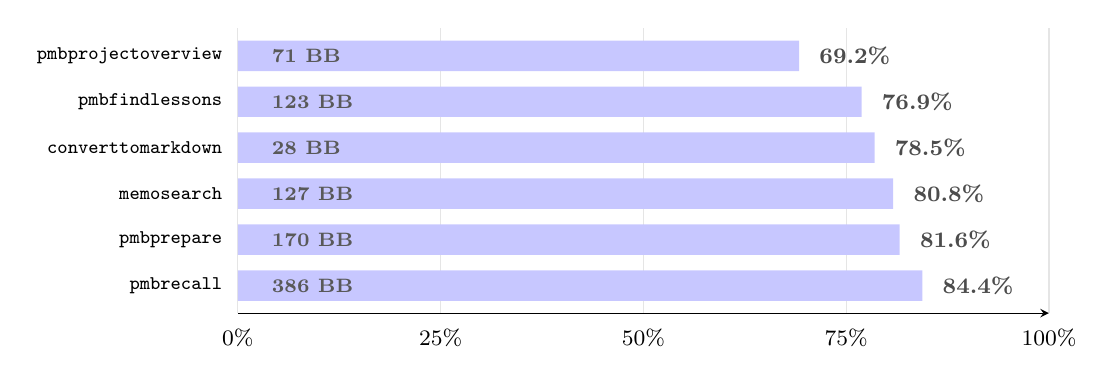
\begin{tikzpicture}

\begin{axis}[
    xbar,
    width=0.98\columnwidth,
    height=5.2cm,
    xmin=0,
    xmax=100,
    ymin=-0.6,
    ymax=5.6,
    y dir=reverse,
    xtick={0,25,50,75,100},
    xticklabels={0\%,25\%,50\%,75\%,100\%},
    ytick={0,1,2,3,4,5},
    yticklabels={
        \texttt{pmbprojectoverview},
        \texttt{pmbfindlessons},
        \texttt{converttomarkdown},
        \texttt{memosearch},
        \texttt{pmbprepare},
        \texttt{pmbrecall}
    },
    bar width=11pt,
    axis x line=bottom,
    axis y line=left,
    y axis line style={draw=none},
    xmajorgrids=true,
    grid style={gray!20},
    tick style={draw=none},
    tick label style={font=\footnotesize},
    yticklabel style={font=\scriptsize},
    clip=true
]

% Bars
\addplot[
    fill=blue!22,
    draw=none
] coordinates {
    (69.2,0)
    (76.9,1)
    (78.5,2)
    (80.8,3)
    (81.6,4)
    (84.4,5)
};

% Number of basic blocks
\node[
    anchor=west,
    font=\scriptsize\bfseries,
    text=black!65
] at (axis cs:3,0) {71 BB};

\node[
    anchor=west,
    font=\scriptsize\bfseries,
    text=black!65
] at (axis cs:3,1) {123 BB};

\node[
    anchor=west,
    font=\scriptsize\bfseries,
    text=black!65
] at (axis cs:3,2) {28 BB};

\node[
    anchor=west,
    font=\scriptsize\bfseries,
    text=black!65
] at (axis cs:3,3) {127 BB};

\node[
    anchor=west,
    font=\scriptsize\bfseries,
    text=black!65
] at (axis cs:3,4) {170 BB};

\node[
    anchor=west,
    font=\scriptsize\bfseries,
    text=black!65
] at (axis cs:3,5) {386 BB};

% Percentages
\node[
    anchor=west,
    font=\footnotesize\bfseries,
    text=black!70
] at (axis cs:70.5,0) {69.2\%};

\node[
    anchor=west,
    font=\footnotesize\bfseries,
    text=black!70
] at (axis cs:78.2,1) {76.9\%};

\node[
    anchor=west,
    font=\footnotesize\bfseries,
    text=black!70
] at (axis cs:79.8,2) {78.5\%};

\node[
    anchor=west,
    font=\footnotesize\bfseries,
    text=black!70
] at (axis cs:82.1,3) {80.8\%};

\node[
    anchor=west,
    font=\footnotesize\bfseries,
    text=black!70
] at (axis cs:82.9,4) {81.6\%};

\node[
    anchor=west,
    font=\footnotesize\bfseries,
    text=black!70
] at (axis cs:85.7,5) {84.4\%};

\end{axis}
\end{tikzpicture}%
}

\caption{Code coverage after 24 hours.}
\Description{Horizontal bar chart of branch coverage reached after 24 hours of fuzzing on each evaluated target, with per-bar percentage labels.}
\label{fig:coverage-tools}
\end{figure}

% TODO(Nazmul): Later, add a bug-discovery effectiveness experiment for the
% semantic vulnerabilities. Under a fixed budget and repeated trials, report
% discovery success and time to discovery for full ToFU and the baseline.
% This is more directly tied to the security contribution than final code
% coverage alone.

% TODO(Nazmul): Later, add a compact ablation summary isolating the
% contributions of sanitizer specialization, LLM and Seed Bank input
% generation, semantic runtime oracles, and coverage-guided mutation.

